---
id: tkz-euclide-ejemplo-30
title: "Circuncentro"
description: "Calcula el circuncentro y traza las tres mediatrices, marcando ángulos rectos y segmentos congruentes."
keywords: [circuncentro, mediatriz, recto, isosceles]
tags: [tkzDefTriangle, tkzDefTriangleCenter,tkzDefLine,tkzGetPoint,tkzMarkRightAngle,mediator]
sort: 30
---
\documentclass[tikz,border=2mm]{standalone}
\usepackage{tkz-base}
\usepackage{tkz-euclide}

\begin{document}
    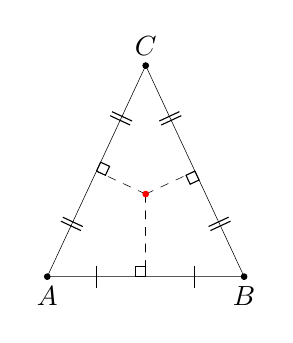
\begin{tikzpicture}[scale=0.5]
        % Define la base AB.
        \tkzDefPoint(0,0){A}
        \tkzDefPoint(5,0){B}

        % Construye el triángulo con dos ángulos iguales (65° y 65°).    
        \tkzDefTriangle[two angles = 65 and 65](A,B)
            \tkzGetPoint{C}

        % Calcula el incentro O (intersección de las mediatrices).
        \tkzDefTriangleCenter[circum](A,B,C)
            \tkzGetPoint{O}

        % Calcula los puntos medios de cada lado
        \tkzDefMidPoint(A,B) \tkzGetPoint{M1}
        \tkzDefMidPoint(B,C) \tkzGetPoint{M2}
        \tkzDefMidPoint(A,C) \tkzGetPoint{M3}    
        
        % Dibuja segmento del punto medio al circuncentro
        \tkzDrawSegment[dashed](O,M1)
        \tkzDrawSegment[dashed](O,M2)
        \tkzDrawSegment[dashed](O,M3)

        % Marca los ángulos rectos
        \tkzMarkRightAngle(A,M1,O)
        \tkzMarkRightAngle(B,M2,O)
        \tkzMarkRightAngle(C,M3,O)

        % Marca segmentos congruentes
        \tkzMarkSegments[mark=|](A,M1 M1,B)
        \tkzMarkSegments[mark=||](A,M3 M3,C C,M2 M2,B)    
        
        % Dibuja el circucentro en rojo                
        \tkzDrawPoints[red](O)

        % Dibuja y etiqueta el resto de los puntos
        \tkzDrawPoints(A,B,C)
        \tkzDrawPolygon(A,B,C)    
        \tkzLabelPoints(A,B)    
        \tkzLabelPoints[above](C)
    \end{tikzpicture}
\end{document}

